\documentclass[11pt, letterpaper]{article}

% Importing packages
\usepackage[left=0.75in, right=0.75in, top=1in, bottom=1in]{geometry}
\usepackage{graphicx}
\usepackage{pdfpages}
\usepackage{hyperref}

\newcommand{\nameA}{Nikhil Sethukumar}
\newcommand{\nameB}{Vishnu Varadan}
\newcommand{\emailA}{nsethukumar@ethz.ch}
\newcommand{\emailB}{vvaradan@ethz.ch}
\newcommand{\rollA}{21-954-029}
\newcommand{\rollB}{21-954-030}  % change!!
\newcommand{\projtitle}{Insert title here}

\title{\projtitle}
\author{\nameA, \nameB}
\hypersetup{
    unicode=true,
    pdftoolbar=false,
    pdfmenubar=false,
    pdffitwindow=false,
    pdftitle={\projtitle},
    pdfauthor={\nameA, \nameB},
    colorlinks=true,
    linkcolor=blue,
    citecolor=magenta,
    urlcolor=cyan
}


\begin{document}
    
\includegraphics[width=2in]{ETHlogo.pdf}

\vspace{\stretch{2}}

\begin{center}

\Large \textsf{Complex Social Systems: Modeling Agents, Learning, and Games}

\textsf{Fall 2022}

\vspace{\stretch{1}}

\normalsize Project Report

\vspace{\stretch{2}}

\textbf{\huge{\projtitle}}

\vspace{\stretch{2}}

\Large{ \nameA, \nameB}

\vspace{\stretch{6}}

\large{
Zurich

\today}

\normalsize

\end{center}
\thispagestyle{empty}

\newpage

    \section*{Agreement for free-download}
    
    \large We hereby agree to make our source code for this project freely available for download from the web pages of the SOMS chair. Furthermore, we assure that all source code is written by ourselves and is not violating any copyright restrictions.

    \vfill

    \hspace*{\stretch{1}} \nameA \hspace*{\stretch{1}} \nameB \hspace*{\stretch{1}}


    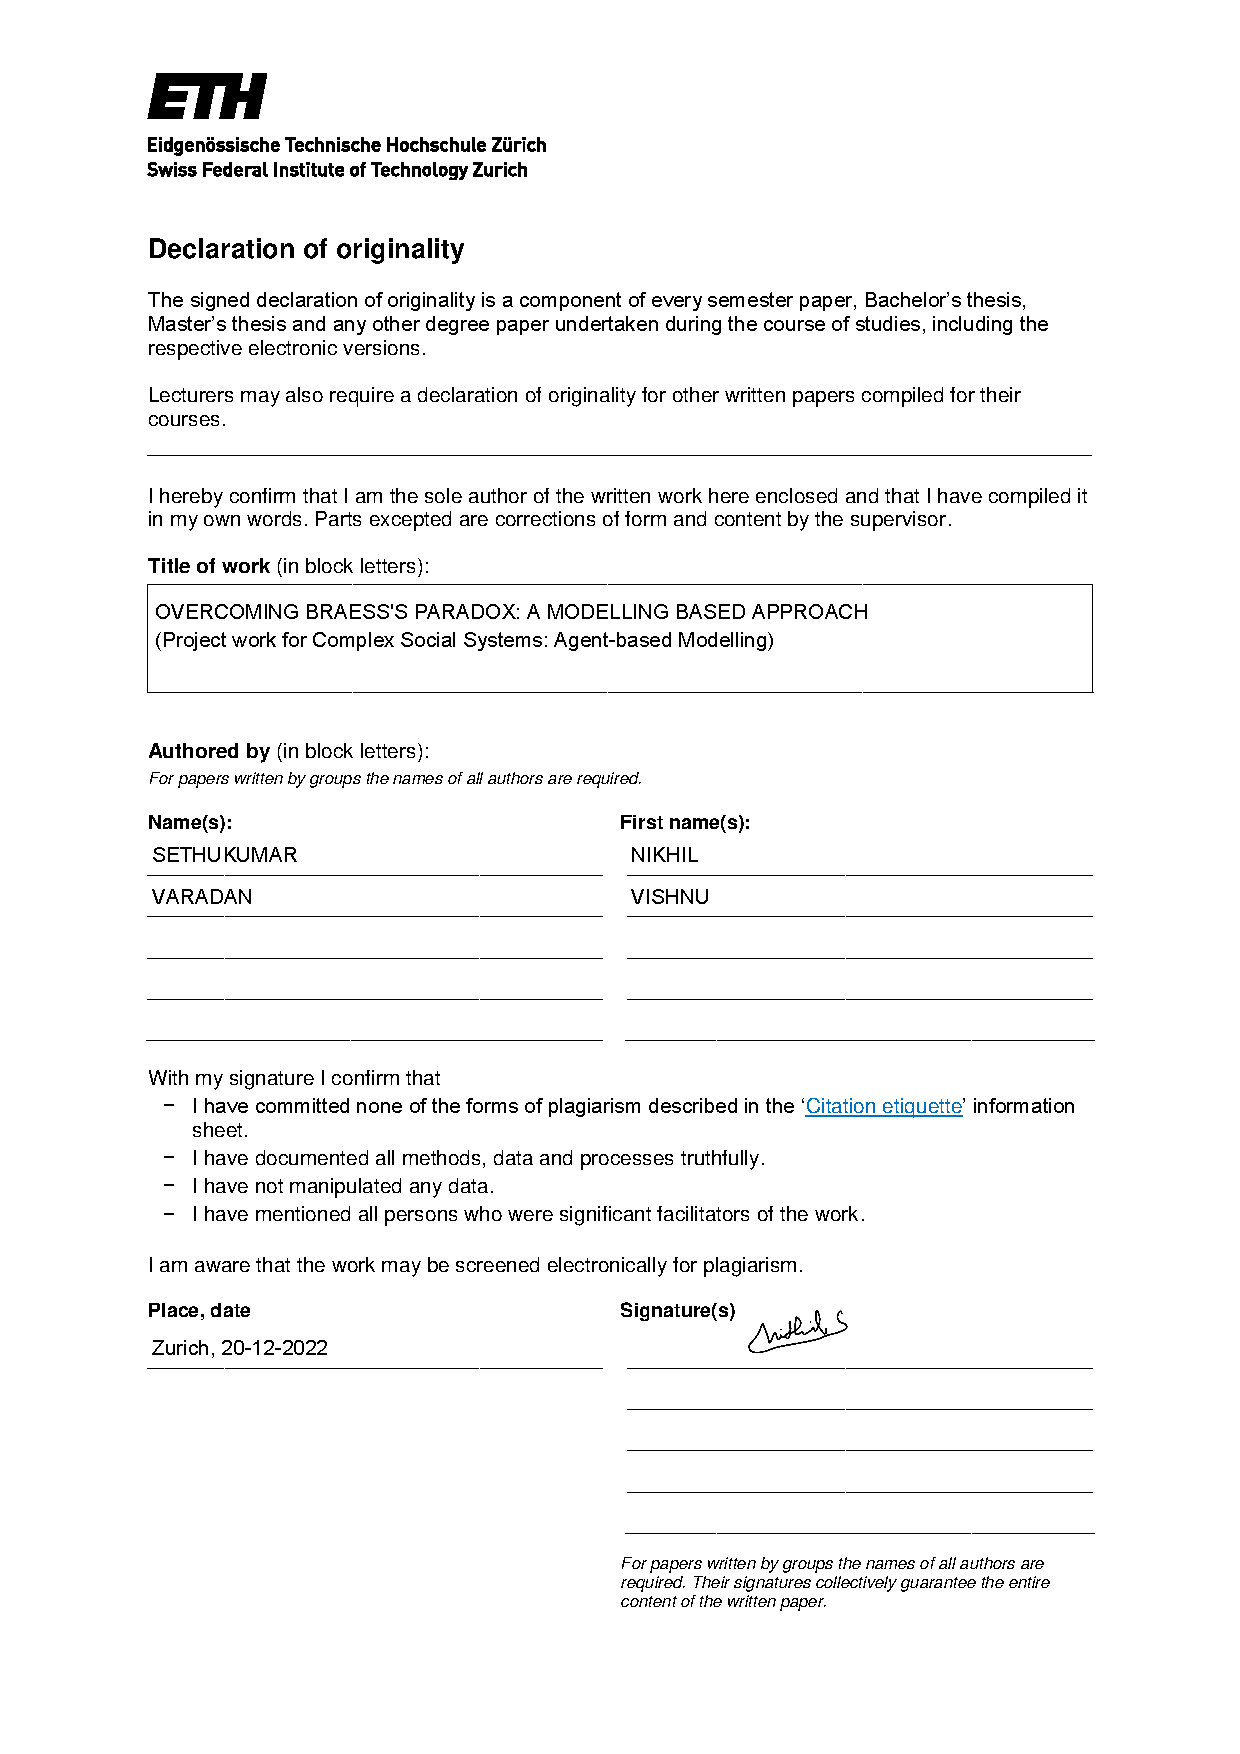
\includepdf{declaration-originality.pdf} % TO BE FILLED
   

    
\tableofcontents

\newpage


\section{Abstract}

\section{Individual contributions}

\section{Introduction and Motivations}

\section{Description of the Model}

\section{Implementation}

\section{Simulation Results and Discussion}

\section{Summary and Outlook}

\section{References}



\end{document}